\documentclass[12pt]{article}

\usepackage[a4paper, margin=1in]{geometry}
\usepackage{amsmath}
\usepackage{array}
\usepackage{tikz}
\usepackage{multicol}
\hyphenpenalty=10000
\exhyphenpenalty=10000
\sloppy
\usepackage[T1]{fontenc}

\setlength{\parindent}{0pt}

\begin{document}

\begin{center}
    {\LARGE Magnetism and Electromagnets}
\end{center}

\vspace{1em}

Magnets produce magnetic fields around them. A magnetic field is the region where magnetic materials or other magnets experience a force. Magnetic field lines are used to show the shape and direction of a magnetic field. Outside of a magnet, magnetic field lines always travel from the north pole to the south pole. The closer the field lines are together, the stronger the magnetic field is in that area. Magnetic field lines never cross each other.

\vspace{1em}

Permanent magnets always produce a magnetic field. Examples include fridge magnets and bar magnets. Electromagnets are different because they only produce a magnetic field when an electric current flows through them. Electromagnets are made by wrapping a coil of wire around an iron core and passing a current through the wire. Electromagnets are useful because they can be switched on and off, and their strength can be changed.

\vspace{1em}

Some magnetic materials can become temporary magnets when placed in a magnetic field. Materials such as iron, nickel, and cobalt can become magnetised when they are brought close to a magnet. This happens because the magnetic field causes tiny magnetic regions inside the material to line up in the same direction. Iron is particularly useful for this because it is easy to magnetise and demagnetise. When the magnetic field is removed, the material may lose most or all of its magnetism. This is why iron is commonly used as the core of electromagnets.

\vspace{1em}

There are several ways to make an electromagnet stronger. Increasing the current in the wire will increase the strength of the magnetic field. Adding more turns of wire around the iron core will also make the electromagnet stronger. Using an iron core instead of an air core greatly increases the strength of the electromagnet.

\vspace{1em}

Magnetic fields can also exert forces on wires carrying electric currents. When a current carrying wire is placed in a magnetic field, a force acts on the wire. This is known as the motor effect. The size of the force can be calculated using the equation:

\[
F = B I l
\]

In this equation, \(F\) is the force in newtons (N), \(B\) is the magnetic flux density in tesla (T), \(I\) is the current in amps (A), and \(l\) is the length of the wire in metres (m).

\vspace{4em}

\textbf{Activity 1}

Read the information above carefully. Write down any key points, important facts, formulas, or definitions into your exercise book.

\newpage

\textbf{Activity 2}

Draw the magnetic field lines around each magnet arrangement below. Include arrows to show the direction of the field.

\vspace{2em}

\textbf{1. Single Bar Magnet}

\vspace{6em}

\begin{center}
\begin{tikzpicture}
\draw (0,0) rectangle (6,1.5);
\draw (3,0) -- (3,1.5);
\node at (1.5,0.75) {\Large N};
\node at (4.5,0.75) {\Large S};
\end{tikzpicture}
\end{center}

\vspace{6em}

\textbf{2. Two Magnets Attracting}

\vspace{6em}

\begin{center}
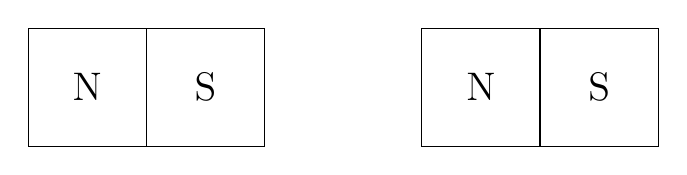
\begin{tikzpicture}
\draw (0,0) rectangle (3,1.5);
\draw (1.5,0) -- (1.5,1.5);
\node at (0.75,0.75) {\Large N};
\node at (2.25,0.75) {\Large S};

\draw (5,0) rectangle (8,1.5);
\draw (6.5,0) -- (6.5,1.5);
\node at (5.75,0.75) {\Large N};
\node at (7.25,0.75) {\Large S};
\end{tikzpicture}
\end{center}

\vspace{6em}

\textbf{3. Two Magnets Repelling}

\vspace{6em}

\begin{center}
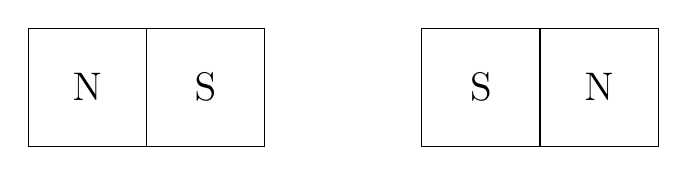
\begin{tikzpicture}
\draw (0,0) rectangle (3,1.5);
\draw (1.5,0) -- (1.5,1.5);
\node at (0.75,0.75) {\Large N};
\node at (2.25,0.75) {\Large S};

\draw (5,0) rectangle (8,1.5);
\draw (6.5,0) -- (6.5,1.5);
\node at (5.75,0.75) {\Large S};
\node at (7.25,0.75) {\Large N};
\end{tikzpicture}
\end{center}

\newpage

\textbf{Activity 3}

Match each keyword to its correct definition.

\vspace{1em}

\begin{minipage}{0.4\textwidth}
\begin{tabular}{|p{6cm}|}
\hline
Magnetic field \\ \hline
Electromagnet \\ \hline
Permanent magnet \\ \hline
Solenoid \\ \hline
Magnetic field line \\ \hline
North pole \\ \hline
South pole \\ \hline
Motor effect \\ \hline
\end{tabular}
\end{minipage}
\hfill
\begin{minipage}{0.45\textwidth}
\begin{tabular}{|p{7cm}|}
\hline
A magnet that only works when current flows \\ \hline
A coil of wire used to create a magnetic field \\ \hline
The region where magnetic forces act \\ \hline
The force produced on a current carrying wire in a magnetic field \\ \hline
The part of a magnet where field lines leave the magnet \\ \hline
A magnet that always produces a magnetic field \\ \hline
A line used to show the direction and shape of a magnetic field \\ \hline
The part of a magnet where field lines enter the magnet \\ \hline
\end{tabular}
\end{minipage}

\vspace{3em}

\textbf{Activity 4}

Fill in the blanks below.

\vspace{1em}

Electromagnets are useful because they can be switched \underline{\hspace{5cm}} and \underline{\hspace{5cm}}.

\vspace{2em}

The strength of an electromagnet can be changed by increasing the \underline{\hspace{4cm}} in the wire.

\vspace{2em}

Adding more \underline{\hspace{6cm}} of wire around the core makes the electromagnet stronger.

\vspace{2em}

Using an \underline{\hspace{6cm}} core increases the strength of the electromagnet.

\vspace{2em}

Permanent magnets always produce a magnetic field, but electromagnets only work when an electric \underline{\hspace{6cm}} flows.

\newpage

\textbf{Activity 5}

Use the equation below to answer the following questions.

\[
F = B I l
\]

\begin{enumerate}
    \item Calculate the force when \(B = 2\,T\), \(I = 3\,A\), and \(l = 0.5\,m\).

    \item Calculate the force when \(B = 1.5\,T\), \(I = 4\,A\), and \(l = 2\,m\).

    \item Calculate the force when \(B = 0.8\,T\), \(I = 5\,A\), and \(l = 0.4\,m\).

    \item Calculate the force when \(B = 3\,T\), \(I = 2\,A\), and \(l = 0.25\,m\).

    \item Calculate the force when \(B = 0.2\,T\), \(I = 10\,A\), and \(l = 1.5\,m\).

    \item Calculate the current when \(F = 6\,N\), \(B = 2\,T\), and \(l = 1\,m\).

    \item Calculate the current when \(F = 12\,N\), \(B = 3\,T\), and \(l = 2\,m\).

    \item Calculate the magnetic flux density when \(F = 10\,N\), \(I = 5\,A\), and \(l = 1\,m\).

    \item Calculate the magnetic flux density when \(F = 8\,N\), \(I = 2\,A\), and \(l = 2\,m\).

    \item Calculate the wire length when \(F = 9\,N\), \(B = 3\,T\), and \(I = 1.5\,A\).

    \item Calculate the force when \(B = 1.2\,T\), \(I = 4\,A\), and \(l = 30\,cm\).

    \item Calculate the force when \(B = 0.5\,T\), \(I = 6\,A\), and \(l = 20\,cm\).

    \item Calculate the current when \(F = 4\,N\), \(B = 2\,T\), and \(l = 40\,cm\).

    \item Calculate the magnetic flux density when \(F = 3\,N\), \(I = 5\,A\), and \(l = 15\,cm\).

    \item Calculate the wire length when \(F = 7.2\,N\), \(B = 4\,T\), and \(I = 3\,A\).
\end{enumerate}

\newpage

\begin{center}
    {\LARGE Answers}
\end{center}

\vspace{1em}

\textbf{Activity 3}

\begin{itemize}
    \item Magnetic field $\rightarrow$ The region where magnetic forces act
    \item Electromagnet $\rightarrow$ A magnet that only works when current flows
    \item Permanent magnet $\rightarrow$ A magnet that always produces a magnetic field
    \item Solenoid $\rightarrow$ A coil of wire used to create a magnetic field
    \item Magnetic field line $\rightarrow$ A line used to show the direction and shape of a magnetic field
    \item North pole $\rightarrow$ The part of a magnet where field lines leave the magnet
    \item South pole $\rightarrow$ The part of a magnet where field lines enter the magnet
    \item Motor effect $\rightarrow$ The force produced on a current carrying wire in a magnetic field
\end{itemize}

\vspace{1em}

\textbf{Activity 4}

\begin{itemize}
    \item on / off
    \item current
    \item turns
    \item iron
    \item current
\end{itemize}

\vspace{1em}

\textbf{Activity 5}

\begin{enumerate}
    \item \(3\,N\)
    \item \(12\,N\)
    \item \(1.6\,N\)
    \item \(1.5\,N\)
    \item \(3\,N\)
    \item \(3\,A\)
    \item \(2\,A\)
    \item \(2\,T\)
    \item \(2\,T\)
    \item \(2\,m\)
    \item \(1.44\,N\)
    \item \(0.6\,N\)
    \item \(5\,A\)
    \item \(4\,T\)
    \item \(0.6\,m\)
\end{enumerate}

\end{document}